\documentclass[ngerman,12pt,parskip=half]{scrartcl}
\usepackage[utf8]{inputenc}
\usepackage{pgf, tikz}
\usepackage{babel}
\usepackage{microtype}
\usepackage{graphicx}
\usepackage{amssymb}
\usepackage{amsmath}
\usepackage[RPvoltages]{circuitikz}
\usetikzlibrary{arrows , automata , positioning , circuits.logic.IEC}



\author{Ann-Christin Falkenreck}
\title {EA2}


\begin{document}
	
\maketitle
\tableofcontents

\section{Aufgabe} 

\begin{center}
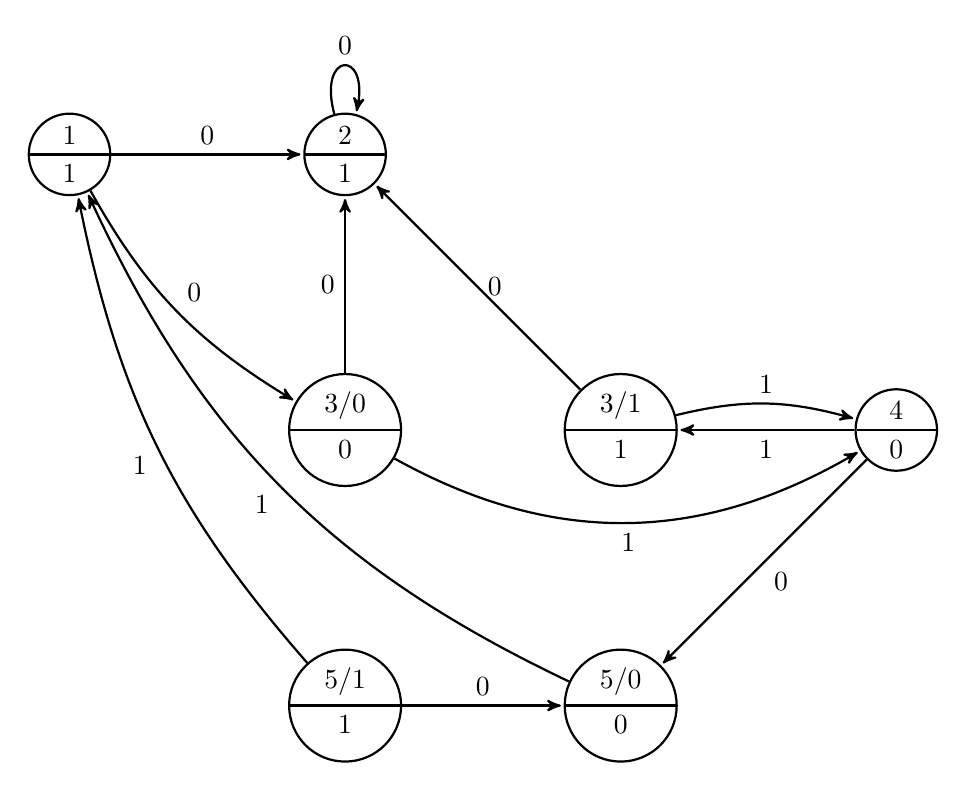
\begin{tikzpicture}[>=stealth',shorten >=1pt,auto,node distance=3.5cm]
%Knoten
\node (1) [state with output, thick] {1 \nodepart{lower} 1};
\node (2) [state with output, thick, right of= 1] {2 \nodepart{lower} 1};
\node (3) [state with output, thick, below of= 2] {3/0 \nodepart{lower} 0};
\node (4) [state with output, thick, right of= 3] {3/1 \nodepart{lower} 1};
\node (5) [state with output, thick, right of= 4] {4 \nodepart{lower} 0};
\node (6) [state with output, thick, below of= 4] {5/0 \nodepart{lower} 0};
\node (7) [state with output, thick, left of= 6] {5/1 \nodepart{lower} 1};

%Verbindungen
\path[thick,->]
(1) edge node {0} (2)
(1) edge [bend angle=15, bend right] node {0} (3)

(2) edge [loop above] node {0} (2)

(3) edge node {0} (2)
(3) edge [bend angle=-30, bend left,below] node {1} (5)

(4) edge [right] node {0} (2)
(4) edge [bend angle=15, bend left] node {1} (5)

(5) edge node {1} (4)
(5) edge node {0} (6)

(6) edge [bend angle=20, bend left] node {1} (1)

(7) edge node {0} (6)
(7) edge [bend angle=15, bend left] node {1} (1)

;
\end{tikzpicture}
\end{center}

\clearpage

\section{Aufgabe} 

\vspace{1.5cm}

\subsection{}
\begin{tabular}{llll}  
	Z & x & Z+ & y \\ \hline	
	0 & 0 & 1 & 1  \\ 
	0 & 1 & 2 & 1 \\ \hline
	1 & 0 & 2 & 1 \\
	1 & 1 & 1 & 0 \\ \hline
	2 & 0 & 2 & 1 \\
	2 & 1 & 0 & 1 \\	 
\end{tabular}

\vspace{1.5cm}

\subsection{}
$Z^+_{0}=Z_{2}x \\
Z^+_{1}=Z_{0}\overline{x}$ v $Z_{1}x \\
Z^+_{2}=Z_{0}x$ v $Z_{1}\overline{x}$ v $Z_{2}\overline{x}$

\vspace{1.5cm}

\subsection{}
\begin{center}
	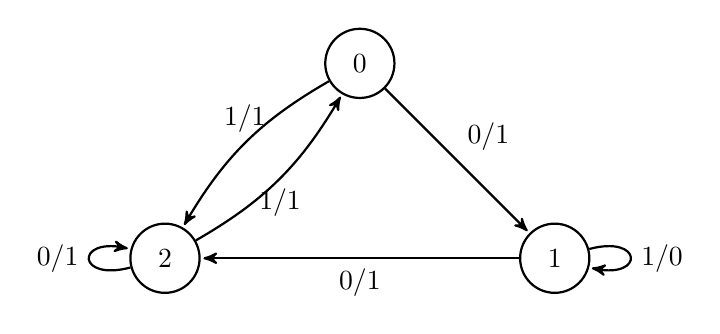
\begin{tikzpicture}[>=stealth',shorten >=1pt,auto,node distance=3.5cm]
	
	%Knoten
	\node (1) [state, thick] {0};
	\node (2) [state, thick, below left of= 1] {2};
	\node (3) [state, thick, below right of= 1] {1};
	
	%Kanten
	\path[thick,->]
	(1)	edge node {0/1} (3)
	(1)	edge [bend angle=15, bend right, above] node {1/1} (2)
	
	(2)	edge [bend angle=15, bend right, below] node {1/1} (1)
	(2)	edge [loop left] node {0/1} (2)
	
	(3)	edge [loop right] node {1/0} (3)
	(3) edge node {0/1} (2);
	
	
	\end{tikzpicture}
\end{center}

\clearpage

\section{Aufgabe} 

\vspace{0,5 cm}

\subsection{}
\begin{tabular}{cccc}  
	$Z_{1}Z_{0}$& x & $Z^+_{1}Z^+_{0}$ & y \\ \hline	
	00 & 0 & 11 & 0  \\ 
	00 & 1 & 01 & 0 \\ \hline
	01 & 0 & 00 & 1 \\
	01 & 1 & 10 & 0 \\ \hline
	10 & 0 & 11 & 1 \\
	10 & 1 & 01 & 0 \\ \hline
	11 & 0 & 00 & 0 \\
	11 & 1 & 10 & 0 \\
\end{tabular}

\vspace{0,5 cm}

\subsection{}
$y=\overline{Z_{1}}Z_{0}x$ v $Z_{1}\overline{Z_{0}}x$ \\
$Z^+_{1}= \overline{Z_{1}}\overline{Z_{0}}\overline{x}$ v x v $Z_{1}Z_0\overline{x}$ \\
$Z^+_{0}=\overline{Z_{1}Z_{0}}x$ v $\overline{Z_{0}}$ v $Z_{1}\overline{Z_{0}x}$

\subsection{}

\begin{center}



\begin{tikzpicture}[scale=1.3, transform shape,circuit logic IEC]

% Koordinaten für Kreuzpunkte
\coordinate (A) at (1,3.5);
\fill (A) circle (2pt);

\coordinate (B) at (3,1.5);
\fill (B) circle (2pt);
\coordinate (C) at (3.25,2.5);
\fill (C) circle (2pt);
\coordinate (D) at (3.5,4);
\fill (D) circle (2pt);

\coordinate (E) at (5,3.5);
\fill (E) circle (2pt);

\coordinate (F) at (6.5,2);
\fill (F) circle (2pt);
\coordinate (G) at (6.75,3);
\fill (G) circle (2pt);
\coordinate (H) at (7,4);
\fill (H) circle (2pt);

\coordinate (I) at (8.5,1.5);
\fill (I) circle (2pt);
\coordinate (J) at (8.75,2.5);
\fill (J) circle (2pt);
\coordinate (K) at (9,3.5);
\fill (K) circle (2pt);

\coordinate (L) at (10.5,2);
\fill (L) circle (2pt);

\coordinate (M) at (12,1.5);
\fill (M) circle (2pt);
\coordinate (N) at (12.25,2);
\fill (N) circle (2pt);
\coordinate (O) at (12.5,4);
\fill (O) circle (2pt);

\coordinate (P) at (4.25,-1);
\coordinate (Q) at (5.5,-1);
\coordinate (R) at (10,-1);
\coordinate (S) at (11,-1);

\coordinate (T) at (0,0);
\coordinate (U) at (0.5,0);
\coordinate (V) at (1,0);
\coordinate (W) at (1.5,0);

\coordinate (X) at (4.5,-6.175);
\fill (X) circle (2pt);

%Eingangsvariabel
\node (x1) at (0,3.5) {$X$};

%Takt
\node (x2) at (4.5,-9) {$C$};

% Gatter
\node[not gate] at ($(x1) + (2,0.5)$) (z1){};

\node[and gate, logic gate inputs=nnn, rotate=270] at ($(B)+(0.25,-1.5)$) (z2) {};
\node[and gate, logic gate inputs=nnn, rotate=270] at ($(F)+(0.25,-2)$) (z4) {};

\node[and gate, logic gate inputs=nnn, rotate=270] at ($(I)+(0.25,-1.5)$) (z5) {};	
\node[and gate, logic gate inputs=nnn, rotate=270] at ($(M)+(0.25,-1.5)$) (z7) {};

\node[or gate, logic gate inputs=nnn, rotate=270] at ($(E)+(0,-5.5)$) (z8) {};
\node[or gate, logic gate inputs=nnn, rotate=270] at ($(L)+(0,-4)$) (z9) {};

\node[flipflop D, rotate=180] at ($(z8)+(-2,-2)$) (D1) {};
\node[flipflop D, rotate=180] at ($(z8)+(-2,-5)$) (D2) {};

% D Flip Flop
\draw (D1.pin 4) node[above] {\tiny$\overline{Z_{1}}$} -|  (W);
\draw (D1.pin 6) node[above] {\tiny$Z_{1}$} -| (V);
\draw (D1.pin 1) node[above] {\tiny$Z^+_{1}$} -| (z8);

\draw (D2.pin 4) node[above] {\tiny$\overline{Z_{0}}$} -| (U);
\draw (D2.pin 6) node[above] {\tiny$Z_{0}$} -| (T);
\draw (D2.pin 1) node[above] {\tiny$Z^+_{0}$} -| (z9);

%Verbindungen von X
\draw(x1.east) -- (K);
\draw (A.east) |- (z1);
\draw(z1) -- (O);

%Verbindungen von C
\draw (D1.pin 3) -| (X);
\draw (D2.pin 3) -- (X);
\draw (X) -| (x2);

%UND Gatter
\draw(B) -| (z2.input 3);
\draw(C) -| (z2.input 2);
\draw(D) -| (z2.input 1);

\draw(F) -| (z4.input 3);
\draw(G) -| (z4.input 2);
\draw(H) -| (z4.input 1);

\draw(I) -| (z5.input 3);
\draw(J) -| (z5.input 2);
\draw(K) -| (z5.input 1);

\draw(M) -| (z7.input 3);
\draw(N) -| (z7.input 2);
\draw(O) -| (z7.input 1);

%ODER Gatter
\draw(z2.output) |- (P);
\draw(P) -| (z8.input 3);
\draw(E) |- (z8.input 2);
\draw(z4.output) |- (Q);
\draw(Q) -| (z8.input 1);

\draw(z5.output) |- (R);
\draw(R) -| (z9.input 3);
\draw(L) |- (z9.input 2);
\draw(z7.output) |- (S);
\draw(S) -| (z9.input 1);

\draw(T) |- (G);
\draw(U) |- (J);
\draw(V) |- (N);
\draw(W) |- (M);

\end{tikzpicture}
\end{center}

\clearpage

\section{Aufgabe} 






\end{document}